\section{Mergeable Types}
\label{sec:mergeable_types}

\begin{figure}

\begin{subfigure}{0.35\textwidth}
\begin{ocaml}
module type MRope = sig
  module A: sig
    type t
    val concat: t -> t -> t
    val split: t -> t*t
    val merge: t -> t -> t -> t
  end
  type t =
  | Leaf of A.t
  | Node of t * int * t
  ... 
  (* Standard rope functions *)
  val merge: t -> t -> t -> t 
end
\end{ocaml}
\caption{Signature of Mergeable Ropes}
\label{fig:mrope-sig}
\end{subfigure}
\begin{subfigure}{0.6\textwidth}
\begin{ocaml}
let rec flatten = function
  | Leaf x -> x
  | Node (l,_,r) -> A.concat (flatten l) (flatten r)

let rec merge old l r =
  if l = r then l else if old = l then r
  else if old = r then l else merge_rec old l r

and merge_rec old l r = match (old,l,r) with
  | Leaf _, _, _ | _, Leaf _, _ 
  | _, _, Leaf _ -> 
      rope_of @@ A.merge (flatten old) 
                    (flatten l) (flatten r)
  | Node (oldl,_,oldr), Node (ll,_,lr), 
    Node (rl,_,rr) ->
      let newl = merge oldl ll rl in
      let newr = merge oldr lr rr in
        Node (newl, create_index newl, newr)
\end{ocaml}
\caption{Mergeable rope implementation}
\label{fig:mrope-merge}
\end{subfigure}

\caption{Signature and implementation for mergeable ropes}
\label{fig:rope}
\end{figure}


The \drawsome example demonstrates the utility of the \name
programming model in building concurrent applications with conceptual
state sharing that make them suitable for transparent deployment in a
distributed setting. The model allows concurrent computations to be
composed around any mergeable type. We now present a series of
examples that demonstrate how mergeable types are built: either by
defining merge functions for ML data types, or by composing existing
mergeable types.

\subsection{Ropes}
\label{sec:ropes}

A rope is a data structure that faciliates efficient implementations
of operations such as concatenation, splitting, lookup and insertion
at a random position etc., for a list of values in a distributed
setting. The values are usually characters, with their lists being
strings. The data structure is a binary tree, whose leaf nodes store
substrings of a larger string such that their left-to-right (in-order)
concatenation yeilds the larger string. The idea is to facilitate
efficient lookups and insertions at random positions in the string by
storing position indexes in the internal nodes of the tree.

Fig.~\ref{fig:mrope-sig} shows a rope interface in OCaml. The type of
the list of values is left abstract (\C{A.t}); it can be instantiated
with any module that supports \C{concat} and \C{split} operations. The
interface shown in Fig.~\ref{fig:mrope-sig} is that of a mergeable
rope (\C{MRope}), whose \C{merge} implementation is shown in
Fig.~\ref{fig:mrope-merge}. The function returns one of its versions
(\C{l} or \C{r}), if the other one is the same as the common
ancestor. Otherwise, it calls \C{merge\_rec}, which recursively
compares the structures of merging ropes, and their common ancestor.
The function recurses until one of the ropes differs from the other
two, or all of them are leaf nodes, at which point it relies on the
(abstract) list merge function (\C{A.merge}) to merge the lists
represented by the ropes. \C{merge\_rec} uses auxiliary functions,
\C{mk\_rope} and \C{create\_index}, whose definitions are not shown to
construct a rope given a list (\C{A.t}), and to compute the index at a
node, given its left sub-tree, resp.

One feature of the mergeable rope implementation that is characterisic
of mergeable types in general is compositionality; a rope is a
polymorphic mergeable data type that composes mergeability over its
polymorphic constituents.   Compositionality is concretized by the
\C{MRope} signature , which requires the type of items in the list
(\C{A.t}) to also be mergeable (\C{A.merge}).

\subsection{Lists}
\label{sec:lists}

\begin{figure}

\begin{subfigure}[b]{0.7\textwidth}
\begin{ocaml}
module type MList = sig
  module A: sig
    type t
    val merge: t -> t -> t -> t
  end
  type t = A.t list
  ... (* All the standard list functions *)
  val merge: t -> t -> t -> t (* and the merge function *)
  (* The following are exposed only for this presentation *)
  type edit = I of A.t * int
    | D of int
    | S of int * A.t * A.t
  val edit_seq: t -> t -> edit list option
  val op_transform: edit list -> edit list -> edit list
end
\end{ocaml}
\caption{Signature of Mergeable Lists}
\label{fig:mlist-sig}
\end{subfigure}


\caption{Mergeable List Implementation}
\label{fig:mlist}
\end{figure}


As an abstract data type, lists support three operations: \C{insert x
  i l}, to insert an element \C{x} at position \C{i} in the list
\C{l}, \C{delete i l}, to delete the element at \C{i}'th position, and
\C{subst i x l}, to substitute the element at the \C{i}'th position
with \C{x}.  Lists of mergeable items are mergeable if they preserve
the following properties:
\begin{itemize}
  \item Elements present in both the merging lists will be present in
  the final list. No element is deleted unless it is deleted in at
  least one list.
  \item An element deleted in one list will not reappear in the merged
  list (unlike, for example, Amazon's replicated shopping cart~\cite{Dynamo}).
  \item The order of elements is retained. That is, if $x$ occurs
  before $y$ in one of the lists, and if both elements are present in
  the merged list, then $x$ occurs before $y$ in the merged list.
\item If an element $y$ is substituted for an element $x$ in one list,
  then $y$ is also substituted for $x$ in the merged list (i.e., $x$
  is absent and $y$ is present), unless $x$ is deleted or substituted
  in the other list. In the former case, deletion wins, and neither
  $x$ nor $y$ occur in the merged list. In the latter case, if $x$ is
  substituted by a different element $z$ in the other list, then the
  merged list substitutes $x$ by a merge of $y$ and $z$, defined as
  per the merge semantics of the list element type.
\end{itemize}

\noindent The merge operation for lists is composed of two separate functions,
\C{edit\_seq} and \C{op\_transform}. Both these functions have been
implemented in less than 50 lines of OCaml included in the appendix.
The functions are described below.
\begin{itemize}
	\item \C{edit\_seq} takes a pair of lists, \C{v} and $\C{v'}$, and computes
		the shortest sequence of list operations that need to be applied on \C{v}
		to obtain \C{v'}. Such a sequence is called an \emph{edit sequence}. The
		length of the sequence corresponds to the standard notion of the \emph{edit
		distance} between the two lists, which can be computed in polynomial
		time~\cite{wagner-fischer}.  \C{edit\_seq} modifies one such algorithm to
		also compute the edit sequence (an \C{edit list}). The implementation
		specified in Fig.~\ref{fig:mlist-sig} represents edits using the type
		\C{edit}.  Constructors \C{I}, \C{D}, and \C{S} stand for \C{insert},
		\C{delete}, and \C{subst}, respectively.\footnote{ Note that \C{I}, \C{D}
		and \C{S} are \emph{not} effects; no list function generates them, and
		they are not exchanged between concurrent threads. They are simply tags
		used by the list merge operation for convenience.  Indeed, to better
		appreciate the virtues of mergeable types, we encourage the reader to
		think about how one might implement a replicated list with this
		functionality using an explicit effect representation as described in
		Sec.~\ref{sec:intro}.}  The subst constructor also carries the \C{A.t}
		element that was substituted. The element serves as the \C{lca} argument to
		\C{A.merge} in case of concurrent conflicting substitutions.
		Fig.~\ref{fig:list-eg} illustrates edit sequences for a sample list.  The
		sequence \C{[I(c,0); S(3,c,s)]} maps the list \C{[a;b;c]} to \C{[c;a;b;s]}
		because \C{subst 3 s (insert c 0 [a;b;c]) = [c;a;b;s]}.
	\item  \C{op\_transform} takes a pair of edit sequences, $s_1$ and $s_2$,
		that map a list $v$ to two different lists, $v_1$ and $v_2$ (e.g.,
		Fig.~\ref{fig:list-eg}), and transforms $s_1$ to $s_1'$ such that $s_1'$
		has the same effect on $v_2$ as $s_1$ had on $v$.  For instance, in
		Fig.~\ref{list-eg}, let $s_1$ be the edit sequence \C{[D(1); S(1,c,d)]},
		which maps the list \C{[a;b;c]} ($v$) to \C{[a;d]} ($v_1$). The \C{D} edit
		deletes the first element of $v$. However, if $s_1$ is to be applied on the
		list \C{[c;a;b;s]} ($v_2$), which has a new element at position 0, the
		\C{D} edit must delete the second element from $v_2$, if it were to
		have the same effect as it did on $v$. We say \C{D(1)} in $s_1$ has to be
		transformed w.r.t the sequence $s_2 = \C{[I(c,0);S(3,c,s)]}$.  The function
		\C{op\_transform} (Fig.~\ref{fig:mlist-sig}) computes such
		\emph{operational transformations} for an edit sequence $s_1$ w.r.t another
		edit sequence $s_2$. A notable transformation rule is for a substitution
		w.r.t another substitution at the same position. Since the substituting
		items could be different, the function relies on the item merge function
		(\C{A.merge}) to merge them into a single item. For instance, in
		Fig.~\ref{fig:list-eg}, there are simultaneous substitutions to the item
		\C{c} in $s_1$ and $s_2$; while $s_1$ substitutes it with \C{d}, $s_2$ does
		it with \C{s}. The merged list therefore substitutes \C{c} with the merge
		of \C{d} and \C{s}, defined as per the merge semantics of \C{A.t}.
\end{itemize}
The \C{MList.merge} can now be defined as a function that first
computes edit sequences, $s_1$ and $s_2$, for the two concurrent
lists, $v_1$ and $v_2$ w.r.t their common ancestor $v$, transforms one
of them (say, $s_1$) w.r.t $s_2$ to obtain $s_1'$, and finally applies
(the operations defined by) $s_1'$ to $v_2$ to obtain the merged list.

\subsection{Lists of Integers and Quantities}.

A mergeable list of integers can be composed using mergeable lists and
mergeable integers.  Concretely, it is a composition of \C{MList} and
\C{Int} types (i.e., \C{MList(Int)}), where \C{Int.merge} is the same
as \C{Counter.merge} (Sec.~\ref{sec:intro}).  An alternative
instantiation of \C{MList} is for a quantity type
(\C{Qty}) that supports \C{add} and \C{subtract} operations, but
\begin{wrapfigure}{l}{.45\textwidth}
  \centering
  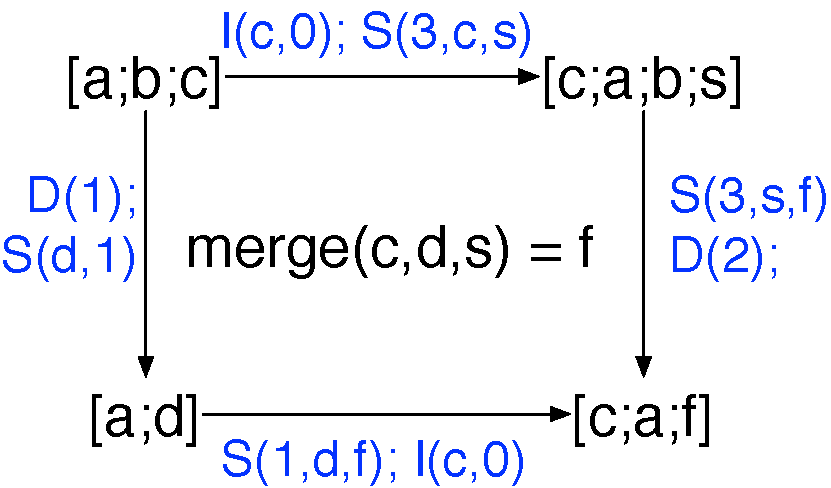
\includegraphics[scale=0.4]{Figures/list-eg}
  \caption{Lists of mergeable values are mergeable. }
  \label{fig:list-eg}
  \vspace*{-.2in}
\end{wrapfigure}
defines its \C{merge} opeation a little differently:
\begin{ocaml}
let merge lca v1 v2 = if v1 = lca then v2
    else (if v2 = lca then v1 else max v1 v2)
\end{ocaml}
\C{MList(Qty)}, like \C{MList(Int)}, is a list of integers, and has
the same semantics under a sequential execution. Their differences
however manifest under a concurrent execution, where both adopt
different methods to reconcile concurrent updates.

If efficient insertions and lookups (by position) are desired over a
large list of integers, while admitting concurrent updates, we require
a mergeable rope of integers, which can be obtained by simply
composing \C{MList(Int)} with \C{MRope} (i.e., \C{MRope(MList(Int))}).

% The mergeable list data type demonstrates a common pattern of writing
% \C{merge} functions applicable to a range of functional data
% structures. For instance, a binary tree (with rotations) can be made
% mergeable in the same way as list, i.e., by computing edit sequences
% (\C{edit\_seq}) and then their transformations
% (\C{op\_transform})\footnote{
%   Like Wagner-Fischer, established algorithms exist for computing tree
%   edit distances~\cite{tree-diff}. An alternative naive method to
%   merge a pair of trees is by merging the lists obtained from their
%   in-order traversal, followed by reconstructing the tree.
% }.

\subsection{Shopping List}

\begin{figure}
\centering
\begin{tabular}{l||l}
\begin{ocaml}
let alice_f : L.t unit t =
  fork bob_f >>= fun () -> (* Invite Bob *)
  get () >>= fun c0 ->
  let qty = L.assoc "eggs" in
  let c0' = L.subst 1 ("eggs",qty+1) c0 in
  sync () ~v:c0' >>=
  fun c1 -> return ()
\end{ocaml}
&
\begin{ocaml}
let bob_f : L.t unit t =
  get () >>= fun c0 ->
  let c0' = L.insert ("candy",Qty.of_int 1) 1 @@
            L.delete @@ L.lookup "eggs" in
  sync () ~v:c0' >>=
  fun c1 -> return ()
\end{ocaml}
\\
\end{tabular}
\caption{Bob and Alice collaboratively build a grocery shopping list}
\label{fig:shopping-list-code}
\end{figure}

A non-trivial demonstration illustrating the compositional power of
mergeable types is shopping list application, that allows its users to
collaboratively build a shopping list (listing items in the decreasing
order of their priority), by adding new items with a
specified quantity, deleting existing items, and increasing or
\begin{wrapfigure}{l}{.5\textwidth}
  \centering
  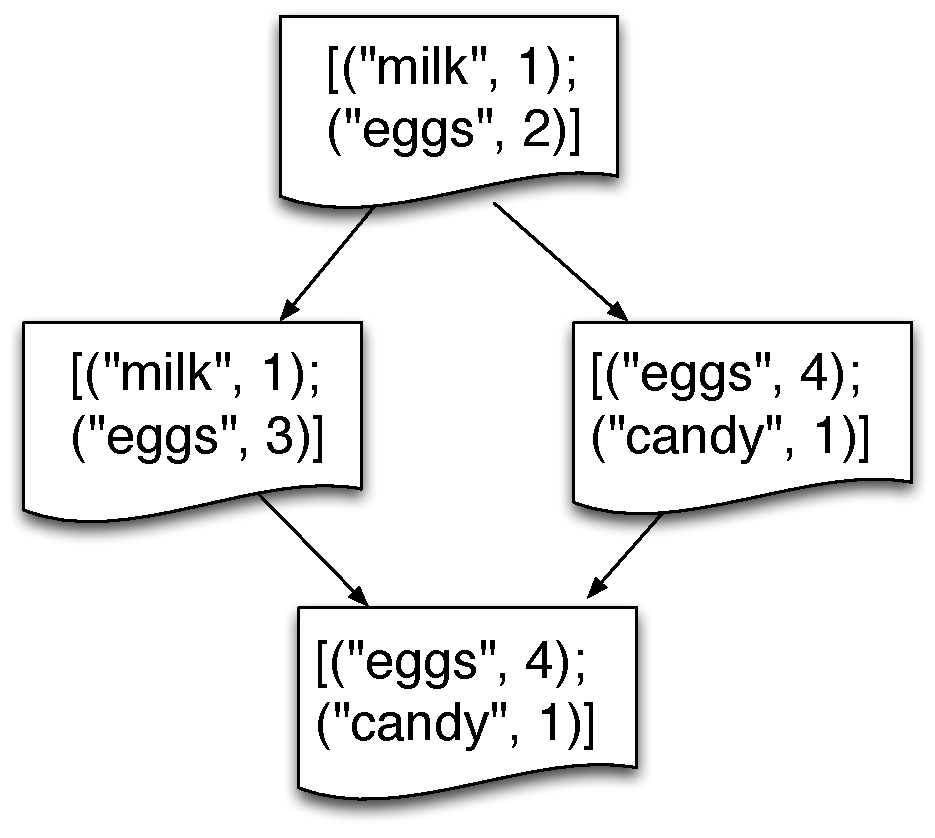
\includegraphics[scale=0.3]{Figures/shopping-list}
  \caption{Merging concurrent shopping lists}
  \label{fig:shopping-list}
  \vspace*{-.2in}
\end{wrapfigure}
decreasing their quantity. An item (\C{Item.t}) is represented as a
tuple of its name (a string) and the quantity (A \C{Qty.t}). The merge
function for \C{Item.t} merges the quantities of items (using
\C{Qty.merge}) having the same names. Items with different names are
considered distinct. A shopping list is a mergeable list of items,
i.e., \C{MList(Item)} (a grocery shopping list may not be large enough
to justify using ropes, but \C{MRope(MList(Item))} is definitely a
possibility).  \C{MList(Item).merge} automatically lifts the merge
semantics for items to merge semantics for lists of items.
Fig.~\ref{fig:shopping-list} illustrates its behavior.  Here, two
users, Alice and Bob, concurrently edit a shopping list whose initial
contents are \C{milk} and \C{eggs}. While both simultaneously update
the quantity of eggs, Bob also removes \C{milk} and inserts \C{candy}.
Fig.~\ref{fig:shopping-list-code} shows the \name code for two
concurrent sessions. The merged shopping list contains \C{eggs} and
\C{candy}, where the quantity of eggs is obtained by merging Alice's
and Bob's quantity as per the definition of \C{Qty.merge}.

The examples described above make certain assumptions about the model
and the underlying system, such as the existence of a single least
common ancestor (LCA) for any pair of versions, the ability to access
a previous version on any branch, and mergeability of any two
concurrent versions. Enforcing these guarantees in a fully
decentralized distributed setting requires addressing non-trivial
theoretical challenges. These, and other details that contribute to
the practicality of our model, such as containing the complexity of
merges, are discussed in subsequent sections.


